\chapter{Metode Penelitian}

Bab ini menjelaskan mengenai metodologi yang digunakan dalam tahap implementasi dan verifikasi \textit{System-on-Chip} (SoC) berbasis \textit{soft-core} mikroprosesor mriscv pada \textit{board} FPGA Digilent Basys3 berbasis chip Xilinx Artix-7, dengan memanfaatkan \textit{open-source synthesis toolchain}. Pembahasan meliputi alat dan bahan yang digunakan, metode yang diterapkan dalam penelitian, alur pelaksanaan tugas akhir, struktur hierarki RTL yang menyusun \textit{soft-core} mriscv, dan metode analisis hasil akhir.


\section{Alat dan Bahan Tugas Akhir}
\label{sec:alat-bahan}

Penelitian tugas akhir ini memanfaatkan kombinasi \textit{hardware} fisik dan \textit{software} untuk melakukan implementasi, verifikasi, serta evaluasi. Rincian mengenai alat dan bahan yang digunakan dalam penelitian ini ditunjukkan sebagai berikut:



\subsection{Alat Tugas Akhir (\textit{Hardware})}
\label{subsec:alat-hardware}

\textit{Hardware} utama yang digunakan sebagai bahan eksperimen meliputi:

\begin{enumerate}
	\item \textit{Board} FPGA Digilent Basys3 dengan chip Xilinx Artix-7 XC7A35T-1CPG236C dengan spesifikasi 33.280 \textit{logic cell}, 1.800 Kbits \textit{Block RAM} internal, dan 50 slot I/O. \textit{Board} ini dilengkapi dengan 16 \textit{switch}, 5 \textit{push button}, \textit{seven-segment display} 4 digit, 16 LED, dan konektor USB untuk pemrograman dan komunikasi serial. Konektor USB tersebut terhubung ke \textit{bridge} USB FTDI FT2232HQ pada \textit{board}. Salah satu \textit{channel}-nya muncul sebagai \textit{virtual COM port} pada komputer dan digunakan untuk komunikasi UART antara \textit{soft-core} dan komputer.
	\item Total Phase Cheetah SPI Adapter sebagai SPI \textit{master} untuk mentransfer \textit{firmware binary} dari PC ke memori mriscv saat \textit{runtime}. \textit{Adapter} ini mendukung \textit{data transfer rate} hingga 40 MHz dan menyediakan \textit{USB interface} untuk komunikasi dengan komputer.
	\item Komputer dengan \textit{operating system} Linux Ubuntu 24.04 LTS atau lebih baru.
\end{enumerate}

\subsection{Bahan Tugas Akhir}
\label{subsec:bahan-tugas-akhir}

Bahan yang digunakan dalam penelitian tugas akhir ini sebagai berikut:

\begin{enumerate}
	\item Yosys Open SYnthesis Suite yang digunakan sebagai \textit{synthesis engine} untuk mentransformasikan deskripsi \textit{Register Transfer Level} (RTL) Verilog menjadi \textit{gate-level netlist} yang tersusun atas \textit{primitive} FPGA Xilinx.
	\item nextpnr-xilinx sebagai \textit{place-and-route tool} (PnR) untuk memetakan \textit{gate-level netlist} ke \textit{physical resource} pada chip FPGA Xilinx Artix-7.
	\item openXC7 Toolchain sebagai \textit{toolchain} untuk mengonversi hasil \textit{place-and-route} menjadi \textit{bitstream file} yang dapat diprogram ke FPGA.
	\item mriscv sebagai \textit{core} mikroprosesor RISC-V yang digunakan sebagai \textit{processing core} utama dalam desain SoC.
	\item openFPGALoader sebagai \textit{software utility} untuk \textit{flashing bitstream} dari PC ke \textit{configuration memory} SRAM FPGA melalui \textit{JTAG interface}.
	\item riscv64-unknown-elf-gcc Toolchain sebagai \textit{toolchain} \textit{cross-compiler} yang mengompilasi \textit{source code} C/C++ menjadi kode \textit{binary} yang dapat dijalankan pada target \textit{instruction set architecture} RISC-V RV32I.
	\item Icarus Verilog (\texttt{iverilog}) sebagai simulator Verilog untuk menjalankan \textit{testbench} fungsional, baik untuk satu modul maupun untuk SoC lengkap yang menjalankan \textit{firmware} hasil kompilasi, sebelum desain disintesis.
	\item \textit{Serial terminal} pada komputer untuk mengirim dan menerima data UART melalui \textit{virtual COM port} dengan \textit{baud rate} 115200.
\end{enumerate}



\section{Metode yang Digunakan}
\label{sec:metode-digunakan}

Perancangan dan penerapan pada penelitian tugas akhir ini dilaksanakan secara langsung, dengan berpusat pada uji coba menggunakan \textit{development board} FPGA sebagai objek eksperimen untuk menguji dan validasi desain \textit{soft-core} mriscv yang telah dimodifikasi untuk berjalan pada \textit{board} FPGA Digilent Basys3. Validitas hasil diperoleh melalui proses sintesis aktual dan pengujian langsung pada \textit{hardware} fisik.

Tahap analisis pada penelitian ini dilakukan melalui dua pendekatan, yaitu analisis validitas fungsional dan analisis kuantitatif terhadap hasil sintesis. Analisis validitas fungsional dilakukan dengan membandingkan perilaku aktual \textit{soft-core} pada \textit{hardware} terhadap perilaku yang diharapkan berdasarkan spesifikasi program yang diunggah, guna memastikan kebenaran implementasi. Analisis kuantitatif dilakukan melalui \textit{benchmarking} terhadap hasil sintesis, mencakup \textit{timing analysis} untuk memperoleh parameter \textit{operating frequency} dan \textit{maximum frequency} (\textit{Fmax}) serta evaluasi \textit{resource utilization} pada FPGA.

\section{Alur Tugas Akhir}
\label{sec:alur-tugas-akhir}

Penulisan tugas akhir ini dilakukan melalui beberapa tahapan yang berlangsung secara berurutan. Kerangka metodologis ini disusun agar setiap tahapan menjadi prasyarat bagi tahapan berikutnya, sehingga proses penelitian dapat ditelusuri secara sistematis.


Penjelasan rinci untuk setiap tahapan diuraikan sebagai berikut.

\begin{enumerate}
	\item \textbf{Studi Literatur dan Analisis RTL \textit{Repository} mriscv}

	Tahap ini diawali dengan studi literatur mengenai arsitektur \textit{soft-core} prosesor RISC-V mriscv, mencakup pemahaman terhadap \textit{instruction set} RV32I \cite{waterman2016riscv}, hierarki modul penyusun \textit{core} (antara lain \textit{control unit} berbasis \textit{multi-cycle finite state machine}, \textit{arithmetic logic unit}, \textit{register file}, dan \textit{memory interface}), serta arsitektur bus AXI4-Lite yang menghubungkan \textit{core} dengan modul periferalnya. Berdasarkan pemahaman tersebut, dilakukan analisis awal terhadap kode RTL \textit{repository} mriscv untuk mengidentifikasi bagian desain yang berpotensi tidak kompatibel dengan \textit{routing fabric} FPGA target, seperti konstruksi bus \textit{tri-state}, struktur \textit{latch}, dan hal lainnya. Hasil analisis ini menjadi dasar penentuan bagian RTL yang perlu dimodifikasi pada tahap berikutnya.

	\item \textbf{Modifikasi dan Implementasi \textit{Hardware}}

	Berdasarkan hasil analisis yang diperoleh, dilakukan modifikasi pada kode RTL yang memerlukan penyesuaian untuk mendukung kompatibilitas antara desain \textit{soft-core} mriscv dengan \textit{routing fabric} FPGA target. Modifikasi yang dilakukan mencakup penyesuaian modul memori SRAM menjadi bentuk \textit{Block RAM} (BRAM) dengan blok inisialisasi nilai awal, penyesuaian struktur modul \textit{interconnect} untuk memastikan \textit{timing} yang andal dan menghindari \textit{timing violation} pada hasil sintesis, serta penggantian struktur bus \textit{tri-state} pada \textit{write-back path} register di dalam \texttt{mriscvcore} dan ALU menjadi struktur \textit{multiplexer} agar dapat disintesis dengan benar pada \textit{routing fabric} FPGA target. Setelah kode RTL dimodifikasi, selanjutnya dilakukan proses sintesis menggunakan \textit{open-source toolchain}, yaitu Yosys untuk menghasilkan \textit{gate-level netlist} dan nextpnr-xilinx untuk proses \textit{place-and-route} pada \textit{board} FPGA Digilent Basys3. Hasil \textit{place-and-route} kemudian dikonversi menjadi \textit{bitstream file} dan diprogramkan ke FPGA menggunakan openFPGALoader.

	Setelah \textit{soft-core} berjalan stabil, rancangan diperluas dengan tiga modul periferal baru yang ditulis dari awal karena tidak tersedia pada \textit{repository} mriscv, yaitu UART \textit{transmitter} (\texttt{uart\_tx.v}), UART \textit{receiver} (\texttt{uart\_rx.v}), dan I2C \textit{master controller} (\texttt{i2c\_master.v}). Ketiga modul dirancang sebagai \textit{slave} AXI4-Lite agar dapat dihubungkan ke \textit{interconnect bus} tanpa mengubah \textit{core}. Setiap modul diverifikasi terlebih dahulu dengan \textit{testbench} pada simulator \texttt{iverilog} sebelum disintesis dan diuji pada \textit{hardware}.

	\item \textbf{Pengembangan \textit{Firmware}}

	Tahap ini mencakup pengembangan \textit{bare-metal firmware} yang berjalan pada \textit{soft-core} mriscv tanpa \textit{operating system}. Pengembangan diawali dengan penyusunan \textit{startup code} yang menyiapkan kondisi awal prosesor sebelum program utama dijalankan, dilanjutkan dengan penyusunan \textit{linker script} untuk mengatur \textit{memory map} program sesuai dengan kapasitas BRAM yang tersedia. Selanjutnya dibuat \textit{header} C yang berfungsi sebagai \textit{hardware abstraction layer} yang memuat fungsi dasar untuk mengakses register periferal, seperti GPIO, UART, dan I2C \textit{controller}. Seluruh kode program dikompilasi menggunakan \textit{toolchain} riscv64-unknown-elf-gcc yang sesuai dengan arsitektur RV32I.

	\item \textbf{Integrasi dan Pengujian Sistem}

	Tahap ini merupakan tahap integrasi antara \textit{hardware} dan \textit{software}, di mana \textit{firmware} yang telah dikompilasi dimuat ke memori \textit{soft-core} mriscv dan diuji secara fungsional. Pada tahap pengembangan awal, \textit{firmware loading} dilakukan dengan menyisipkan kode \textit{binary} hasil kompilasi langsung ke dalam parameter inisialisasi (\texttt{INIT\_FILE}) modul BRAM pada tahap sintesis RTL, sehingga untuk mengubah kode yang berjalan pada \textit{soft-core} mriscv diperlukan proses sintesis ulang dari awal secara menyeluruh.

	Setelah dipastikan bahwa \textit{hardware} dan \textit{software} telah berjalan dengan baik, selanjutnya ditambahkan mekanisme \textit{runtime loader} dengan \textit{Serial Peripheral Interface} (SPI) menggunakan Total Phase Cheetah SPI Adapter. Mekanisme ini memungkinkan \textit{firmware} yang telah dikompilasi dimuat ke memori \textit{soft-core} mriscv tanpa perlu melakukan sintesis ulang \textit{hardware} setiap kali ingin dilakukan perubahan program.

	Selanjutnya, dilakukan pengujian fungsional menggunakan modul \textit{rotary encoder} KY-040 sebagai \textit{input device}, dan OLED SSD1306 sebagai \textit{output device} yang berkomunikasi dengan \textit{soft-core} mriscv melalui protokol I2C. Komunikasi I2C dengan layar OLED diuji dengan dua cara, yaitu secara \textit{bit-bang} melalui GPIO dan melalui \textit{hardware} I2C \textit{controller}. UART \textit{interface} diuji dengan mengirim teks dari \textit{soft-core} ke \textit{serial terminal} pada komputer serta melakukan \textit{echo} terhadap karakter yang diterima dari terminal. Pengujian dilakukan untuk memastikan bahwa seluruh skenario pengujian berjalan sesuai dengan yang diharapkan, mencakup \textit{firmware loading}, eksekusi instruksi RV32I, pembacaan arah putaran dari \textit{rotary encoder}, pengendalian tampilan pada layar OLED, serta pertukaran data melalui UART.

	\item \textbf{Pengumpulan Data dan Analisis}

	Tahap terakhir adalah pengumpulan data dan analisis hasil implementasi. Tahap ini diawali dengan validasi fungsional untuk memastikan seluruh skenario pengujian pada tahap sebelumnya berjalan sesuai dengan yang diharapkan. Selanjutnya dilakukan \textit{benchmarking} terhadap hasil sintesis, yang mencakup evaluasi \textit{resource utilization} FPGA seperti \textit{Look-Up Table} (LUT), \textit{Flip-Flop} (FF), dan \textit{Block RAM} (BRAM), serta \textit{timing analysis} untuk memperoleh nilai \textit{maximum frequency} (\textit{Fmax}) yang dapat dicapai oleh desain. Data yang diperoleh dari kedua proses tersebut selanjutnya dianalisis dan dibahas secara mendalam pada bab selanjutnya.
\end{enumerate}

\pagebreak

\section{Struktur Hierarki \textit{Soft-core} mriscv}
\label{sec:struktur-hierarki}

Subbab ini menguraikan struktur hierarki rancangan RTL (\textit{Register Transfer Level}) yang menyusun \textit{soft-core} mriscv, mulai dari \textit{central processing unit} (CPU \texttt{mriscvcore}) beserta komponen-komponen penyusunnya seperti \textit{Arithmetic Logic Unit} (ALU) dan \textit{register file}, \textit{interconnect bus}, hingga modul periferal yang digunakan pada penelitian ini.

% Uraian pada subbab ini bersifat struktural untuk memberikan gambaran menyeluruh mengenai rancangan yang dijadikan basis pengembangan; rincian teknis mengenai modifikasi pada tiap modul dibahas secara terpisah pada Bab IV.

\subsection{Hierarki Modul RTL Verilog}
\label{subsec:hierarki-modul-rtl}

Secara keseluruhan, modul RTL pada \textit{repository} mriscv tersusun atas tiga \textit{layer} hierarki, yaitu \textit{chip layer}, \textit{core layer}, dan \textit{layer} modul fungsional penyusun \textit{core}. Susunan hierarki tersebut ditunjukkan sebagai berikut.

\dirtree{%
	.1 \texttt{impl\_axi.v}.
	.2 \texttt{mriscvcore.v}.
	.3 \texttt{FSM.v}.
	.3 \texttt{DECO\_INSTR.v}.
	.3 \texttt{ALU.v}.
	.3 \texttt{REG\_FILE.v}.
	.3 \texttt{MEMORY\_INTERFACE.v}.
	.3 \texttt{MULT.v}.
	.3 \texttt{IRQ.v}.
	.3 \texttt{UTILITY.v}.
	.2 \texttt{spi\_axi\_master.v}.
	.2 \texttt{axi4\_interconnect.v}.
	.2 \texttt{AXI\_SP32B1024.v}, \texttt{SP32B1024.v}.
	.2 \texttt{DAC\_interface\_AXI.v}.
	.2 \texttt{ADC\_interface\_AXI.v}.
	.2 \texttt{completogpio.v} (GPIO \textit{bank} 1).
	.2 \texttt{spi\_axi\_slave.v}.
	.2 \texttt{uart\_tx.v}.
	.2 \texttt{uart\_rx.v}.
	.2 \texttt{completogpio.v} (GPIO \textit{bank} 2).
	.2 \texttt{i2c\_master.v}.
}

Gambar \ref{fig:hierarki-rtl} menunjukkan hierarki yang sama dalam bentuk diagram blok, beserta hubungan setiap modul melalui bus AXI4-Lite. Notasi S0 sampai S8 pada gambar menyatakan \textit{slave} ke-0 sampai ke-8, dan nama pada gambar adalah nama modul Verilog tanpa ekstensi \texttt{.v}.

\begin{figure}[H]
	\centering
	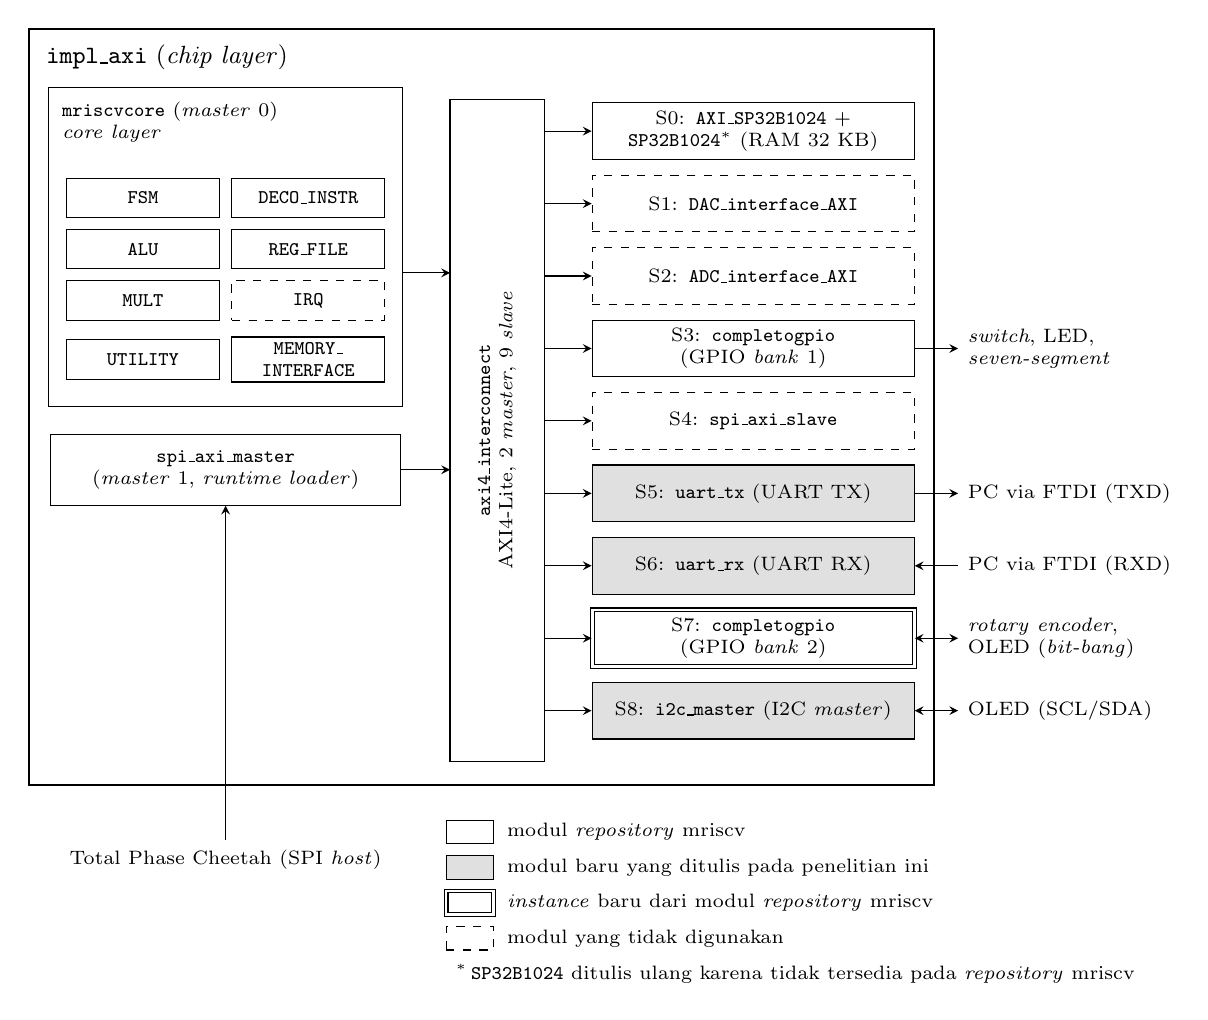
\begin{tikzpicture}[
		>=stealth,
		mod/.style={draw, rectangle, align=center, font=\scriptsize, inner sep=2pt},
		sub/.style={mod, minimum height=0.5cm, text width=1.8cm},
		slv/.style={mod, minimum height=0.72cm, text width=3.95cm},
		baru/.style={fill=black!12},
		inst/.style={double, double distance=1pt},
		idle/.style={dashed},
		ext/.style={font=\scriptsize, anchor=west, align=left}
	]
		% chip layer
		\draw[thick] (0,0) rectangle (11.5,-9.6);
		\node[anchor=north west, font=\small] at (0.1,-0.08) {\texttt{impl\_axi} (\textit{chip layer})};

		% core layer: mriscvcore.v beserta modul fungsional
		\draw (0.25,-0.75) rectangle (4.75,-4.8);
		\node[anchor=north west, font=\scriptsize, align=left] at (0.3,-0.8) {\texttt{mriscvcore} (\textit{master} 0)\\\textit{core layer}};
		\node[sub] at (1.45,-2.15) {\texttt{FSM}};
		\node[sub] at (3.55,-2.15) {\texttt{DECO\_INSTR}};
		\node[sub] at (1.45,-2.8) {\texttt{ALU}};
		\node[sub] at (3.55,-2.8) {\texttt{REG\_FILE}};
		\node[sub] at (1.45,-3.45) {\texttt{MULT}};
		\node[sub, idle] at (3.55,-3.45) {\texttt{IRQ}};
		\node[sub] at (1.45,-4.2) {\texttt{UTILITY}};
		\node[sub] at (3.55,-4.2) {\texttt{MEMORY\_}\\\texttt{INTERFACE}};

		% master 1
		\node[mod, minimum height=0.9cm, text width=4.3cm] (spim) at (2.5,-5.6) {\texttt{spi\_axi\_master}\\(\textit{master} 1, \textit{runtime loader})};

		% interconnect
		\draw (5.35,-0.9) rectangle (6.55,-9.3);
		\node[rotate=90, font=\scriptsize, align=center] at (5.95,-5.1) {\texttt{axi4\_interconnect}\\AXI4-Lite, 2 \textit{master}, 9 \textit{slave}};
		\coordinate (icL) at (5.35,0);
		\coordinate (icR) at (6.55,0);
		\draw[->] (4.75,-3.1) -- (icL |- 0,-3.1);
		\draw[->] (spim.east) -- (icL |- spim.east);

		% slave
		\node[slv] (s0) at (9.2,-1.3) {S0: \texttt{AXI\_SP32B1024} +\\\texttt{SP32B1024}$^{*}$ (RAM 32 KB)};
		\node[slv, idle] (s1) at (9.2,-2.22) {S1: \texttt{DAC\_interface\_AXI}};
		\node[slv, idle] (s2) at (9.2,-3.14) {S2: \texttt{ADC\_interface\_AXI}};
		\node[slv] (s3) at (9.2,-4.06) {S3: \texttt{completogpio}\\(GPIO \textit{bank} 1)};
		\node[slv, idle] (s4) at (9.2,-4.98) {S4: \texttt{spi\_axi\_slave}};
		\node[slv, baru] (s5) at (9.2,-5.9) {S5: \texttt{uart\_tx} (UART TX)};
		\node[slv, baru] (s6) at (9.2,-6.82) {S6: \texttt{uart\_rx} (UART RX)};
		\node[slv, inst] (s7) at (9.2,-7.74) {S7: \texttt{completogpio}\\(GPIO \textit{bank} 2)};
		\node[slv, baru] (s8) at (9.2,-8.66) {S8: \texttt{i2c\_master} (I2C \textit{master})};
		\foreach \s in {s0,s1,s2,s3,s4,s5,s6,s7,s8}
			\draw[->] (icR |- \s.west) -- (\s.west);

		% external device
		\draw[->] (s3.east) -- ++(0.55,0) node[ext] {\textit{switch}, LED,\\\textit{seven-segment}};
		\draw[->] (s5.east) -- ++(0.55,0) node[ext] {PC via FTDI (TXD)};
		\draw[<-] (s6.east) -- ++(0.55,0) node[ext] {PC via FTDI (RXD)};
		\draw[<->] (s7.east) -- ++(0.55,0) node[ext] {\textit{rotary encoder},\\OLED (\textit{bit-bang})};
		\draw[<->] (s8.east) -- ++(0.55,0) node[ext] {OLED (SCL/SDA)};
		\draw[->] (2.5,-10.3) -- (spim.south);
		\node[below, font=\scriptsize] at (2.5,-10.3) {Total Phase Cheetah (SPI \textit{host})};

		% legenda
		\node[mod, minimum width=0.6cm, minimum height=0.3cm] at (5.6,-10.2) {};
		\node[ext] at (5.95,-10.2) {modul \textit{repository} mriscv};
		\node[mod, baru, minimum width=0.6cm, minimum height=0.3cm] at (5.6,-10.65) {};
		\node[ext] at (5.95,-10.65) {modul baru yang ditulis pada penelitian ini};
		\node[mod, inst, minimum width=0.6cm, minimum height=0.3cm] at (5.6,-11.1) {};
		\node[ext] at (5.95,-11.1) {\textit{instance} baru dari modul \textit{repository} mriscv};
		\node[mod, idle, minimum width=0.6cm, minimum height=0.3cm] at (5.6,-11.55) {};
		\node[ext] at (5.95,-11.55) {modul yang tidak digunakan};
		\node[ext] at (5.3,-12.0) {$^{*}$\,\texttt{SP32B1024} ditulis ulang karena tidak tersedia pada \textit{repository} mriscv};
	\end{tikzpicture}
	\caption{Diagram Hierarki Modul RTL dan Hubungannya melalui Bus AXI4-Lite}
	\label{fig:hierarki-rtl}
\end{figure}

Modul \texttt{impl\_axi.v} merupakan \textit{chip layer} yang menjadi \textit{wrapper} instansiasi bagi seluruh modul utama pada struktur hierarki di atas, mulai dari \textit{core} mriscv, SPI \textit{interface} untuk \textit{runtime loader}, \textit{interconnect bus}, hingga modul-modul periferal, yang seluruhnya saling terhubung melalui bus AXI4-Lite.

Modul \texttt{mriscvcore.v} merupakan \textit{central processing unit} (CPU) sekaligus sebagai \textit{master} bus ke-0. Modul ini tersusun atas beberapa modul fungsional, antara lain \texttt{FSM.v} yang berfungsi sebagai \textit{control unit} berbasis \textit{multi-cycle finite state machine}, \texttt{DECO\_INSTR.v} sebagai \textit{decoder} instruksi RV32I, \texttt{ALU.v} sebagai \textit{arithmetic logic unit}, \texttt{REG\_FILE.v} sebagai \textit{register file}, \texttt{MEMORY\_INTERFACE.v} sebagai \textit{memory/bus interface} untuk instruksi \textit{load}/\textit{store}, \texttt{MULT.v} sebagai \textit{multiplier}, \texttt{IRQ.v} sebagai unit \textit{timer-based interrupt}, dan \texttt{UTILITY.v} sebagai unit instruksi \textit{utility}/sistem.

Selain \texttt{mriscvcore.v}, terdapat beberapa modul penyusun lain pada \textit{chip layer}. Modul \texttt{spi\_axi\_master.v} berfungsi sebagai SPI \textit{interface} sekaligus \textit{master} bus ke-1. Modul ini berperan sebagai \textit{runtime loader} yang menghubungkan \textit{soft-core} dengan Total Phase Cheetah SPI Adapter (sebagai \textit{host} eksternal) untuk memuat program ke dalam modul memori. Selanjutnya, modul \texttt{axi4\_interconnect.v} bertindak sebagai \textit{interconnect bus} AXI4-Lite yang menghubungkan kedua \textit{master} tersebut dengan sembilan modul \textit{slave}. Lima \textit{slave} pertama merupakan bagian dari desain asli mriscv, meliputi \texttt{AXI\_SP32B1024.v} dan \texttt{SP32B1024.v} sebagai modul memori (\textit{slave} ke-0), \texttt{DAC\_interface\_AXI.v} sebagai DAC \textit{interface} (\textit{slave} ke-1, tidak digunakan pada penelitian ini), \texttt{ADC\_interface\_AXI.v} sebagai ADC \textit{interface} (\textit{slave} ke-2, tidak digunakan pada penelitian ini), \texttt{completogpio.v} sebagai modul GPIO (\textit{slave} ke-3), dan \texttt{spi\_axi\_slave.v} sebagai SPI \textit{master interface} yang dikendalikan \textit{core} untuk mengirim data ke perangkat SPI eksternal (\textit{slave} ke-4, tidak digunakan pada penelitian ini). Seluruh modul untuk kelima \textit{slave} tersebut berasal dari \textit{repository} mriscv, kecuali \texttt{SP32B1024.v} yang tidak tersedia pada \textit{repository} sehingga ditulis ulang pada penelitian ini (Subbab \ref{subsec:sp32b1024}). Empat \textit{slave} berikutnya ditambahkan pada penelitian ini. Tiga di antaranya merupakan modul baru yang ditulis pada penelitian ini, yaitu \texttt{uart\_tx.v} sebagai UART \textit{transmitter} (\textit{slave} ke-5), \texttt{uart\_rx.v} sebagai UART \textit{receiver} (\textit{slave} ke-6), dan \texttt{i2c\_master.v} sebagai I2C \textit{master controller} (\textit{slave} ke-8). \textit{Slave} ke-7 merupakan instansiasi kedua \texttt{completogpio.v} dari \textit{repository} mriscv yang dipakai sebagai GPIO \textit{bank} 2.

\subsection{Struktur Internal \texttt{mriscvcore}}
\label{subsec:struktur-internal-mriscvcore}

\textit{Processing unit} utama pada mriscv, yaitu \texttt{mriscvcore.v}, bekerja berdasarkan arsitektur \textit{multi-cycle} yang dikendalikan oleh \textit{control unit} \texttt{FSM.v}. \textit{Control unit} ini tersusun atas tujuh \textit{state} yang dieksekusi berurutan untuk setiap instruksi: \textit{fetch}, \textit{decode}, \textit{execute}, dan \textit{memory access}. Ditambahkan pula \textit{wait state} pada tahap \textit{fetch} dan \textit{memory access} untuk mengakomodasi latensi BRAM yang bersifat \textit{synchronous}, serta satu \textit{state} \textit{trap} yang menghentikan eksekusi secara permanen ketika ditemukan instruksi ilegal atau \textit{bus error}. Karena bersifat \textit{multi-cycle} dan tidak menerapkan \textit{pipeline}, setiap instruksi membutuhkan lebih dari satu \textit{clock cycle} untuk selesai dieksekusi (\textit{Cycles Per Instruction}/CPI $>1$). Oleh karena itu, \textit{hazard control unit} antarinstruksi tidak diperlukan pada arsitektur ini \cite{harris2021digital, solovev2021asmd}.

\texttt{DECO\_INSTR.v} menerjemahkan instruksi yang telah diambil pada tahap \textit{fetch} untuk menentukan jenis operasi dan operand yang digunakan. Operand tersebut diambil dari \texttt{REG\_FILE.v}, \textit{register file} yang menyimpan 32 register 32-\textit{bit} sesuai spesifikasi arsitektur RV32I. \texttt{ALU.v} menangani komputasi aritmetika dan logika, sementara akses ke memori maupun periferal pada bus berlangsung melalui \texttt{MEMORY\_INTERFACE.v}. \texttt{MULT.v} menangani instruksi perkalian \texttt{mul}, \texttt{mulh}, \texttt{mulhsu}, dan \texttt{mulhu} dari ekstensi Zmmul menggunakan \textit{Booth multiplier} iteratif. Seperti \texttt{ALU.v}, \texttt{MULT.v} diaktifkan oleh sinyal \texttt{enable\_exec} dari \texttt{FSM.v} pada tahap \textit{execute}. Bedanya, perkalian membutuhkan beberapa \textit{clock cycle}, sehingga logika pada \texttt{mriscvcore.v} baru menyatakan tahap \textit{execute} selesai (\texttt{done\_exec}) setelah \texttt{MULT.v} mengeluarkan sinyal \textit{done}. Dengan demikian, \textit{core} mriscv mendukung RV32I ditambah ekstensi Zmmul, yaitu perkalian tanpa pembagian. \textit{Firmware} bawaan pada penelitian ini dikompilasi dengan \texttt{-march=rv32i}, sehingga operator perkalian pada kode C dijalankan oleh rutin \textit{software} \texttt{\_\_mulsi3}. Instruksi perkalian \textit{hardware} baru dipakai bila \textit{firmware} dikompilasi dengan \texttt{-march=rv32i\_zmmul}. \textit{Repository} mriscv juga menyertakan \texttt{IRQ.v} untuk penanganan \textit{interrupt timer}, tetapi \textit{output interrupt}-nya tidak disambungkan pada \texttt{impl\_axi.v}, sehingga \texttt{IRQ.v} tidak dipakai pada penelitian ini. \textit{Output} dari kelima modul tersebut, yaitu \texttt{ALU.v}, \texttt{MEMORY\_INTERFACE.v}, \texttt{MULT.v}, \texttt{IRQ.v}, dan \texttt{UTILITY.v}, digabungkan melalui satu \textit{shared bus} menuju \texttt{REG\_FILE.v} untuk proses \textit{write-back}.

Gambar \ref{fig:struktur-mriscvcore} menunjukkan hubungan antarmodul fungsional di dalam \texttt{mriscvcore.v}. Garis tebal horizontal menyatakan bus operand (\texttt{rs1}, \texttt{rs2}, \texttt{imm}, dan \texttt{code}) yang dibagikan ke seluruh unit eksekusi dan \texttt{MEMORY\_INTERFACE.v}, sedangkan simpul OR menyatakan penggabungan \textit{output} unit-unit tersebut menjadi sinyal \texttt{rd} yang ditulis kembali ke \texttt{REG\_FILE.v}. Nama sinyal pada gambar mengikuti nama \textit{wire} pada \texttt{mriscvcore.v}.

\begin{figure}[H]
	\centering
	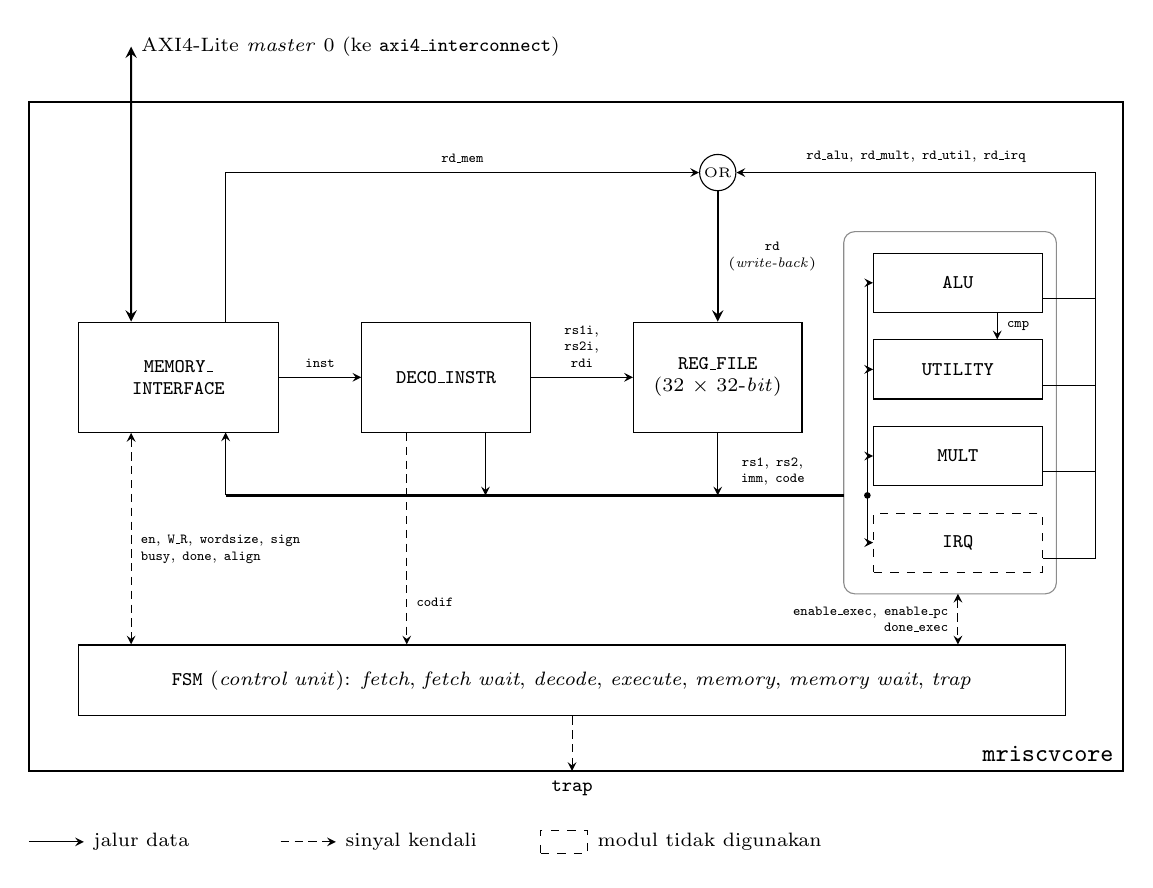
\begin{tikzpicture}[
		>=stealth,
		mod/.style={draw, rectangle, align=center, font=\scriptsize, inner sep=2pt},
		unit/.style={mod, minimum height=0.75cm, text width=2.0cm},
		idle/.style={dashed},
		ctl/.style={densely dashed, <->},
		lbl/.style={font=\tiny, align=center}
	]
		% batas core
		\draw[thick] (-1.9,3.5) rectangle (12.0,-5.0);
		\node[anchor=south east, font=\small] at (12.0,-5.0) {\texttt{mriscvcore}};

		% blok datapath
		\node[mod, minimum height=1.4cm, text width=2.4cm] (mem) at (0,0) {\texttt{MEMORY\_}\\\texttt{INTERFACE}};
		\node[mod, minimum height=1.4cm, text width=2.0cm] (deco) at (3.4,0) {\texttt{DECO\_INSTR}};
		\node[mod, minimum height=1.4cm, text width=2.0cm] (reg) at (6.85,0) {\texttt{REG\_FILE}\\(32 $\times$ 32-\textit{bit})};

		% unit eksekusi
		\node[unit] (alu)  at (9.9,1.2)  {\texttt{ALU}};
		\node[unit] (mult) at (9.9,-1.0)  {\texttt{MULT}};
		\node[unit] (util) at (9.9,0.1) {\texttt{UTILITY}};
		\node[unit, idle] (irq) at (9.9,-2.1) {\texttt{IRQ}};
		\draw[black!45, rounded corners] (8.45,1.85) rectangle (11.15,-2.75);

		% FSM
		\node[mod, minimum height=0.9cm, text width=12.4cm] (fsm) at (5.0,-3.85)
			{\texttt{FSM} (\textit{control unit}): \textit{fetch}, \textit{fetch wait}, \textit{decode}, \textit{execute}, \textit{memory}, \textit{memory wait}, \textit{trap}};

		% AXI4-Lite
		\draw[<->, thick] ([xshift=-0.6cm]mem.north) -- (-0.6,4.2)
			node[right, font=\scriptsize] {AXI4-Lite \textit{master} 0 (ke \texttt{axi4\_interconnect})};

		% inst dan indeks register
		\draw[->] (mem.east) -- node[above, lbl] {\texttt{inst}} (deco.west);
		\draw[->] (deco.east) -- node[above, lbl] {\texttt{rs1i},\\\texttt{rs2i},\\\texttt{rdi}} (reg.west);

		% bus operand
		\draw[very thick] (0.6,-1.5) -- (8.45,-1.5);
		\node[lbl, anchor=south] at (7.55,-1.5) {\texttt{rs1}, \texttt{rs2},\\\texttt{imm}, \texttt{code}};
		\draw[->] (reg.south) -- (reg.south |- 0,-1.5);
		\draw[->] ([xshift=0.5cm]deco.south) -- ([xshift=0.5cm]deco.south |- 0,-1.5);
		\draw[->] (0.6,-1.5) -- (0.6,-0.7);
		\foreach \u in {alu,util,mult,irq}
			\draw[->] (8.75,0 |- \u.west) -- (\u.west);
		\draw (8.75,-1.5 |- alu.west) -- (8.75,-1.5 |- irq.west);
		\fill (8.75,-1.5) circle (1.2pt);

		% cmp ALU -> UTILITY
		\draw[->] ([xshift=0.5cm]alu.south) -- node[right, lbl] {\texttt{cmp}} ([xshift=0.5cm]util.north);

		% shared bus rd (write-back)
		\foreach \u in {alu,util,mult,irq}
			\draw ([yshift=-0.2cm]\u.east) -- ([yshift=-0.2cm]\u.east -| 11.65,0);
		\draw ([yshift=-0.2cm]irq.east -| 11.65,0) -- (11.65,2.6);
		\node[draw, circle, inner sep=1pt, font=\tiny] (or) at (6.85,2.6) {OR};
		\draw[->] (11.65,2.6) -- node[above, lbl] {\texttt{rd\_alu}, \texttt{rd\_mult}, \texttt{rd\_util}, \texttt{rd\_irq}} (or.east);
		\draw[->] ([xshift=0.6cm]mem.north) |- node[pos=0.75, above, lbl] {\texttt{rd\_mem}} (or.west);
		\draw[->, thick] (or.south) -- node[right, lbl] {\texttt{rd}\\(\textit{write-back})} (reg.north);

		% sinyal kendali FSM
		\draw[ctl] ([xshift=-0.6cm]mem.south) -- ([xshift=-0.6cm]mem.south |- fsm.north)
			node[pos=0.55, right, lbl, align=left] {\texttt{en}, \texttt{W\_R}, \texttt{wordsize}, \texttt{sign}\\\texttt{busy}, \texttt{done}, \texttt{align}};
		\draw[densely dashed, ->] ([xshift=-0.5cm]deco.south) -- ([xshift=-0.5cm]deco.south |- fsm.north)
			node[pos=0.8, right, lbl] {\texttt{codif}};
		\draw[ctl] (9.9,-2.75) -- (9.9,0 |- fsm.north)
			node[pos=0.5, left, lbl, align=right] {\texttt{enable\_exec}, \texttt{enable\_pc}\\\texttt{done\_exec}};
		\draw[densely dashed, ->] (fsm.south) -- (5.0,-5.0) node[below, font=\scriptsize] {\texttt{trap}};

		% legenda
		\draw[->] (-1.9,-5.9) -- ++(0.7,0) node[right, font=\scriptsize] {jalur data};
		\draw[densely dashed, ->] (1.3,-5.9) -- ++(0.7,0) node[right, font=\scriptsize] {sinyal kendali};
		\node[mod, idle, minimum width=0.6cm, minimum height=0.3cm] at (4.9,-5.9) {};
		\node[right, font=\scriptsize] at (5.2,-5.9) {modul tidak digunakan};
	\end{tikzpicture}
	\caption{Diagram Blok Struktur Internal \texttt{mriscvcore}}
	\label{fig:struktur-mriscvcore}
\end{figure}

\subsection{Bus AXI4-Lite dan Modul Periferal}
\label{subsec:bus-axi4-periferal}

Seluruh modul pada \textit{chip layer} saling terhubung melalui \texttt{axi4\_interconnect.v}, \textit{interconnect bus} bertipe AXI4-Lite yang menghubungkan dua \textit{master} dan sembilan \textit{slave}. \texttt{mriscvcore.v} bertindak sebagai \textit{master} ke-0 dan \texttt{spi\_axi\_master.v} sebagai \textit{master} ke-1, sedangkan kesembilan \textit{slave} beserta \textit{address map}-nya ditunjukkan pada Tabel \ref{Tab: Peta Alamat AXI}. \textit{Address} pada tabel merupakan \textit{word address} (32-\textit{bit}). \textit{Byte address} yang dipakai \textit{firmware} sama dengan empat kali \textit{word address}.

\begin{table}[h]
	\centering
	\begin{tabular}{|c|l|c|p{5.5cm}|}
		\hline
		\textbf{Slave} & \textbf{Periferal} & \textbf{\textit{Word Address}} & \textbf{Keterangan} \\
		\hline
		0 & Memori (RAM) & \texttt{0x0000}--\texttt{0x1FFF} & Digunakan untuk penyimpanan program dan data \\ \hline
		1 & DAC & \texttt{0x4000}--\texttt{0x4001} & Tidak digunakan pada penelitian ini \\ \hline
		2 & ADC & \texttt{0x4008}--\texttt{0x4009} & Tidak digunakan, \textit{output} ditetapkan nol \\ \hline
		3 & GPIO \textit{bank} 1 & \texttt{0x4010}--\texttt{0x401F} & \textit{Switch}, LED, dan \textit{seven-segment} \\ \hline
		4 & SPI \textit{interface} & \texttt{0x04000000} & Tidak digunakan pada penelitian ini \\ \hline
		5 & UART TX & \texttt{0x4020} & UART \textit{transmitter} (ditambahkan) \\ \hline
		6 & UART RX & \texttt{0x4021} & UART \textit{receiver} (ditambahkan) \\ \hline
		7 & GPIO \textit{bank} 2 & \texttt{0x4030}--\texttt{0x403F} & \textit{Rotary encoder} dan \textit{line} I2C OLED secara \textit{bit-bang} (ditambahkan) \\ \hline
		8 & I2C \textit{master} & \texttt{0x4040}--\texttt{0x4043} & \textit{Hardware} I2C \textit{controller} (ditambahkan) \\ \hline
	\end{tabular}
	\vspace{0.5em}
	\caption{\textit{Address Map} Bus AXI4-Lite}
	\label{Tab: Peta Alamat AXI}
\end{table}

\textit{Slave} ke-0 merupakan modul memori yang tersusun atas \texttt{AXI\_SP32B1024.v} sebagai \textit{bus interface} dan \texttt{SP32B1024.v} sebagai modul memori yang dipetakan ke \textit{Block RAM} (BRAM) FPGA untuk menyimpan program \textit{firmware} beserta data selama eksekusi. \textit{Slave} ke-1 dan ke-2 masing-masing adalah DAC \textit{interface} dan ADC \textit{interface} yang tersedia pada \textit{repository} mriscv, tetapi tidak dimanfaatkan pada penelitian ini karena tidak ada kebutuhan \textit{analog signal processing}. \textit{Slave} ke-4, \texttt{spi\_axi\_slave.v}, merupakan SPI \textit{master interface} yang memungkinkan \textit{core} mengirim data ke perangkat SPI eksternal. \textit{Output}-nya tidak dihubungkan ke pin \textit{board}, sehingga modul ini juga tidak digunakan. Modul ini berbeda dari \textit{SPI runtime loader}: \texttt{spi\_axi\_master.v} berkedudukan sebagai \textit{master} ke-1 yang menulis \textit{firmware} langsung ke memori (\textit{slave} ke-0) tanpa melalui \texttt{mriscvcore.v}.

Modul \texttt{completogpio.v} merupakan modul periferal \textit{input-output} digital (GPIO) yang diinstansiasi dua kali. Instansiasi pertama (\textit{slave} ke-3, GPIO \textit{bank} 1) terhubung ke \textit{switch}, LED, dan \textit{seven-segment} pada \textit{board}. Instansiasi kedua (\textit{slave} ke-7, GPIO \textit{bank} 2) ditambahkan agar \textit{external device} tidak berbagi indeks pin dengan \textit{bank} 1. Dua pin \textit{input} \textit{bank} 2 membaca sinyal CLK dan DT dari \textit{rotary encoder} KY-040, yang didekode dengan metode \textit{quadrature decoding} berbasis \textit{software}, sedangkan dua pin \textit{output}-nya men-\textit{drive} \textit{line} SCL dan SDA layar OLED SSD1306 untuk komunikasi I2C secara \textit{bit-bang}.

Komunikasi serial dengan komputer ditangani oleh \texttt{uart\_tx.v} (\textit{slave} ke-5) dan \texttt{uart\_rx.v} (\textit{slave} ke-6), yang terhubung ke \textit{channel} serial USB pada \textit{board}. Modul \texttt{i2c\_master.v} (\textit{slave} ke-8) menyediakan \textit{hardware} I2C \textit{controller} yang memakai \textit{line} SCL dan SDA yang sama dengan GPIO \textit{bank} 2, sehingga layar OLED dapat dikendalikan secara \textit{bit-bang} maupun melalui \textit{hardware controller} tanpa mengubah \textit{circuit}. Rancangan ketiga modul tersebut diuraikan pada Subbab \ref{subsec:rancangan-uart-i2c}.

\subsection{Rancangan Modul Periferal UART dan I2C}
\label{subsec:rancangan-uart-i2c}

Modul \texttt{uart\_tx.v}, \texttt{uart\_rx.v}, dan \texttt{i2c\_master.v} ditulis dari awal sebagai \textit{slave} AXI4-Lite dengan pola \textit{interface} yang sama: \textit{write channel} dan \textit{read channel} masing-masing dikendalikan oleh FSM kecil yang menyelesaikan setiap transaksi bus dalam beberapa \textit{clock cycle}. Pola ini disebut \textit{non-blocking}. Pengiriman satu \textit{byte} UART dengan \textit{baud rate} 115200 memakan sekitar 4.340 \textit{clock cycle} pada \textit{clock core}, tetapi transaksi AXI ke modul tetap selesai dalam beberapa \textit{cycle}, sehingga periferal yang lambat tidak menahan \textit{interconnect bus} yang juga dipakai \textit{SPI runtime loader}. Proses menunggu periferal siap dipindahkan ke \textit{firmware}, yang melakukan \textit{polling} terhadap \textit{bit} status \textit{busy} sebelum menulis data berikutnya. Data yang ditulis ketika modul masih \textit{busy} akan diabaikan. Ketiga modul menerima parameter \texttt{CLK\_HZ} yang harus sama dengan frekuensi \textit{clock core} (50 MHz), karena \textit{baud rate} UART dan frekuensi SCL I2C diturunkan dari parameter tersebut.

Modul \texttt{uart\_tx.v} mengirim data dengan format 8N1 (8 \textit{bit} data, \textit{no parity}, 1 \textit{stop bit}) secara LSB-\textit{first} dengan \textit{baud rate} tetap 115200. \textit{Bit period} sebesar $\lfloor 50\,000\,000/115\,200 \rfloor = 434$ \textit{clock cycle}, sehingga \textit{baud rate} aktual 115.207 dengan \textit{error} sekitar 0,0064\%. \textit{Transmitter} dikendalikan FSM dengan empat \textit{state} (IDLE, START, DATA, STOP). \textit{Output} TXD dihubungkan ke pin A18 \textit{board}.

Modul \texttt{uart\_rx.v} menerima data dengan format yang sama melalui pin B18. Sinyal RXD yang bersifat \textit{asynchronous} terhadap \textit{clock core} dilewatkan \textit{two-flip-flop synchronizer}. Setelah \textit{falling edge} \textit{start bit} terdeteksi, \textit{receiver} menunggu setengah \textit{bit period} lalu memeriksa ulang RXD. Bila RXD sudah kembali \textit{high}, pulsa tersebut dianggap \textit{glitch} dan diabaikan. Setiap \textit{bit} data kemudian di-\textit{sample} pada \textit{mid-bit}, dan \textit{stop bit} yang bernilai nol dicatat sebagai \textit{framing error}. \textit{Byte} yang diterima disimpan pada \textit{holding register} satu \textit{byte} bersama tiga \textit{flag}: \textit{valid}, \textit{overrun} (ada \textit{byte} yang tertimpa sebelum sempat dibaca), dan \textit{framing error}. Pembacaan register sekaligus melakukan \textit{clear} terhadap ketiga \textit{flag} tersebut.

Modul \texttt{i2c\_master.v} merupakan I2C \textit{master controller} \textit{byte-level}. Satu penulisan ke register CMD menjalankan satu operasi dengan urutan tetap: [START atau \textit{repeated} START] $\rightarrow$ [kirim satu \textit{byte} atau terima satu \textit{byte}] $\rightarrow$ [STOP], dengan setiap bagian dipilih melalui \textit{bit} pada CMD. Setiap \textit{bit} I2C dibagi menjadi empat \textit{phase}, dan panjang satu \textit{phase} ditentukan register DIV dalam satuan \textit{clock cycle}. Nilai \textit{default}-nya 31, sehingga frekuensi SCL sekitar 400 kHz (\textit{Fast-mode}). \textit{Controller} ini membaca ACK/NACK dari \textit{slave}, mendukung \textit{clock stretching} (\textit{controller} menunggu SCL benar-benar \textit{high} sebelum melanjutkan), dan mendeteksi \textit{arbitration lost}.

\textit{Line} SCL dan SDA dibangun sebagai \textit{open-drain} pada \textit{top module} dengan logika \textit{wired-AND}: \textit{line} bernilai \textit{low} apabila salah satu dari GPIO \textit{bank} 2 atau \texttt{i2c\_master.v} men-\textit{drive low}, dan bernilai \textit{high} melalui \textit{pull-up} apabila keduanya melakukan \textit{release}. Dengan cara ini \textit{firmware} I2C \textit{bit-bang} yang sudah ada tetap dapat dipakai tanpa \textit{multiplexer} tambahan. Konsekuensinya, karena GPIO \textit{bank} 2 bernilai nol setelah \textit{reset}, \textit{firmware} yang memakai \textit{hardware controller} harus menulis logika 1 ke kedua pin GPIO \textit{bank} 2 terlebih dahulu. \textit{Register map} ketiga modul ditunjukkan pada Tabel \ref{Tab: Register UART I2C}.

\begin{table}[htbp]
	\centering
	\small
	\begin{tabular}{|l|c|c|p{7.2cm}|}
		\hline
		\textbf{Modul} & \textbf{\textit{Byte Address}} & \textbf{Akses} & \textbf{Fungsi} \\
		\hline
		UART TX & \texttt{0x10080} & \textit{Write} & \texttt{[7:0]}: \textit{byte} yang dikirim \\ \cline{3-4}
		 & & \textit{Read} & \texttt{[0]}: \textit{busy} \\ \hline
		UART RX & \texttt{0x10084} & \textit{Read} & \texttt{[7:0]}: data, \texttt{[8]}: \textit{valid}, \texttt{[9]}: \textit{overrun}, \texttt{[10]}: \textit{framing error}. \textit{Flag} di-\textit{clear} saat dibaca \\ \hline
		I2C DATA & \texttt{0x10100} & \textit{Write}/\textit{Read} & \textit{Write}: \textit{byte} yang dikirim. \textit{Read}: \textit{byte} terakhir yang diterima \\ \hline
		I2C CMD & \texttt{0x10104} & \textit{Write} & \texttt{[0]} START, \texttt{[1]} STOP, \texttt{[2]} WRITE, \texttt{[3]} READ, \texttt{[4]} NACK setelah \textit{byte} yang dibaca \\ \hline
		I2C STATUS & \texttt{0x10108} & \textit{Read} & \texttt{[0]}: \textit{busy}, \texttt{[1]}: NACK dari \textit{slave}, \texttt{[2]}: \textit{arbitration lost} \\ \hline
		I2C DIV & \texttt{0x1010C} & \textit{Write}/\textit{Read} & Jumlah \textit{clock cycle} per seperempat periode SCL (minimum 4, \textit{default} 31) \\ \hline
	\end{tabular}
	\normalsize
	\vspace{0.5em}
	\caption{\textit{Register Map} Modul UART dan I2C}
	\label{Tab: Register UART I2C}
\end{table}

Verifikasi ketiga modul dilakukan dalam tiga \textit{level}. \textit{Level} pertama adalah \textit{unit testbench} pada \texttt{iverilog} untuk setiap modul, mencakup kondisi normal dan kondisi \textit{error} seperti \textit{overrun}, \textit{framing error}, \textit{glitch}, NACK, \textit{clock stretching}, dan \textit{arbitration lost}. \textit{Level} kedua adalah simulasi SoC lengkap, yaitu \textit{testbench} yang memuat \textit{firmware} hasil kompilasi melalui \textit{frame} SPI lalu menjalankannya pada \textit{core} mriscv. \textit{Level} ketiga adalah pengujian pada \textit{board} menggunakan \textit{firmware} uji, dengan hasil diamati melalui \textit{serial terminal}, LED, layar OLED, dan LED indikator \textit{trap} (LD15).

\section{Metode Analisis Hasil Akhir}
\label{sec:metode-analisis-hasil-akhir}

Analisis terhadap hasil akhir penelitian ini dilakukan melalui dua pendekatan, yaitu analisis fungsional dan analisis kuantitatif terhadap hasil sintesis.

\subsection{Analisis Fungsional}
\label{subsec:analisis-fungsional}

Analisis fungsional dilakukan dengan membandingkan perilaku aktual sistem terhadap perilaku yang diharapkan pada lima sasaran pengujian. Pada GPIO \textit{interface} untuk LED, kebenaran fungsional diukur dari kesesuaian pola nyala LED yang dihasilkan \textit{firmware} terhadap pola yang telah ditentukan pada program yang diunggah. Pada \textit{seven-segment display}, kebenaran fungsional diukur dari kesesuaian digit yang ditampilkan terhadap nilai yang seharusnya ditampilkan berdasarkan \textit{firmware} uji yang dijalankan.

Pada sasaran pengujian menggunakan \textit{rotary encoder} KY-040, kebenaran fungsional diukur dari kesesuaian arah putaran (\textit{CW}/\textit{CCW}) yang terbaca oleh \textit{firmware} melalui metode \textit{quadrature decoding} terhadap arah putaran fisik yang sebenarnya dilakukan pada \textit{encoder}. Pada layar OLED SSD1306, kebenaran fungsional diukur dari kesesuaian tampilan pada layar terhadap data yang dikirimkan oleh \textit{firmware} melalui protokol I2C, baik secara \textit{bit-bang} maupun melalui \textit{hardware} I2C \textit{controller}, mencakup keberhasilan inisialisasi layar maupun kesesuaian karakter atau grafik yang ditampilkan. Untuk \textit{hardware} I2C \textit{controller}, kriteria ditambah dengan status ACK yang dibaca langsung oleh \textit{hardware} pada setiap \textit{byte}: selama pengujian tidak boleh ada \textit{byte} yang dijawab NACK maupun kejadian \textit{arbitration lost}.

Pada UART \textit{interface}, kebenaran fungsional \textit{transmitter} diukur dari kesesuaian teks yang diterima \textit{serial terminal} pada komputer terhadap \textit{string} yang dikirim \textit{firmware}, termasuk pada pengiriman terus-menerus tanpa jeda. Kebenaran fungsional \textit{receiver} diukur dari kesesuaian karakter hasil \textit{echo} oleh \textit{firmware} terhadap karakter yang diketik pada terminal. Implementasi dinyatakan berhasil secara fungsional apabila \textit{output} sistem pada kelima sasaran pengujian tersebut sesuai dengan hasil yang diharapkan. Apabila ditemukan ketidaksesuaian pada salah satu sasaran pengujian, dilakukan penelusuran lebih lanjut terhadap penyebabnya.

\subsection{Analisis Kuantitatif}
\label{subsec:analisis-kuantitatif}

Analisis kuantitatif dilakukan terhadap dua parameter utama hasil sintesis, yaitu \textit{maximum operating frequency} (\textit{Fmax}) dan \textit{resource utilization} FPGA. Nilai \textit{Fmax} diperoleh dari laporan \textit{timing analysis} yang dihasilkan oleh nextpnr-xilinx pada setiap proses sintesis. Nilai \textit{Fmax} dicetak dua kali pada log \textit{output} nextpnr-xilinx, sehingga nilai yang diambil sebagai data adalah laporan kedua yang bersifat final setelah tahap \textit{routing} selesai. Karena proses \textit{place-and-route} pada nextpnr-xilinx bersifat stokastik terhadap nilai \textit{seed} yang digunakan \cite{darvishi2025pipeline}, analisis dilakukan melalui dua skema eksperimen. Skema pertama adalah pengujian \textit{repeatability}, yaitu proses sintesis diulang beberapa kali pada konfigurasi \textit{seed} yang sama, untuk menguji konsistensi hasil pada kondisi \textit{place-and-route} yang deterministik. Skema kedua adalah pengujian sensitivitas \textit{seed}, yaitu proses sintesis diulang menggunakan beberapa nilai \textit{seed} eksplisit yang berbeda, untuk menguji variabilitas nilai \textit{Fmax} yang dapat timbul akibat proses \textit{placement} dan \textit{routing} yang berbeda pada RTL yang sama. Nilai \textit{Fmax} rata-rata dan standar deviasi dari kedua skema tersebut selanjutnya dibandingkan terhadap \textit{target operating frequency} sistem, guna menentukan \textit{safety margin} desain.

\textit{Resource utilization} FPGA dianalisis berdasarkan \textit{post-synthesis report} yang dihasilkan oleh Yosys \cite{shah2019yosys}, yang memuat statistik pemakaian \textit{Look-Up Table} (LUT), \textit{Flip-Flop} (FF), dan \textit{Block RAM} (BRAM), dinyatakan dalam jumlah pemakaian pada chip FPGA Xilinx Artix-7 XC7A35T. Analisis ini turut digunakan untuk mengevaluasi efisiensi implementasi desain, termasuk perbandingan \textit{resource utilization} antara konfigurasi kapasitas memori yang berbeda.

Biaya \textit{resource} modul periferal UART dan I2C yang ditambahkan dievaluasi dengan dua cara. Pertama, setiap modul disintesis secara \textit{standalone} menggunakan \texttt{synth\_xilinx} pada Yosys untuk memperoleh jumlah LUT dan FF milik modul tersebut. Kedua, utilisasi keseluruhan desain setelah penambahan periferal dibandingkan dengan utilisasi konfigurasi sebelumnya. Nilai \textit{Fmax} desain akhir juga diperiksa kembali untuk memastikan \textit{operating frequency} 50 MHz tetap terpenuhi setelah penambahan periferal.


% \subsection{Tahap Modifikasi \textit{Repository}}

% Bagian ini menjelaskan prosedur modifikasi \textit{repository} mriscv yang dilakukan untuk menyesuaikan dengan target implementasi pada board FPGA Digilent Basys3. Modifikasi ini mencakup perubahan pada file konfigurasi, penyesuaian RTL seperti penambahan atau penghapusan modul sesuai kebutuhan penelitian.

% \subsubsection{Modifikasi RTL}

% Modifikasi RTL meliputi penyesuaian pada tingkat deskripsi RTL Verilog untuk memastikan kompatibilitas dengan target FPGA, termasuk perubahan pada jalur sinyal (\textit{port} pada Verilog), penyesuaian blok logika, dan pengaturan ulang modul untuk meloloskan \textit{design rule check} (DRC) oleh nextpnr-xilinx dan menjaga kestabilan pada implementasi FPGA.

% modul \texttt{SP32B1024.v} ditulis ulang karena tidak tersedia pada \textit{repository} mriscv. Modul ini menyertakan blok \textit{initialization} untuk mencegah kondisi \textit{undefined} pada memori saat \textit{power-up}.

% % \noindent pada modul \texttt{axi4\_interconnect.v}, dilakukan modifikasi sebagai berikut:

% Modul \texttt{axi4\_interconnect.v} pada RTL \textit{repository upstream} menggunakan blok kombinasional dengan \textit{sensitivity list} eksplisit (\texttt{always @(m\_axi\_awvalid[unpk\_idx] or RST or m\_axi\_awaddr[...])}) yang menghasilkan struktur \textit{latch}. Hal tersebut berpotensi untuk menjadi resiko \textit{timing violation} pada implementasi FPGA, karena sifatnya yang tidak sinkron terhadap sinyal clock. Dilakukan modifikasi sebagai berikut:

% % --- BAGIAN BEFORE ---
% \noindent\textbf{BEFORE (upstream \texttt{onchipuis/mriscv})}
% \begin{lstlisting}[language=Verilog]
% // Phase 1 - Convert to latched array
% generate
%     for (unpk_idx=0; unpk_idx<(masters); unpk_idx=unpk_idx+1) begin
%         always @(m_axi_awvalid[unpk_idx] or RST or m_axi_awaddr[((sword)*unpk_idx+(sword-1)):((sword)*unpk_idx)]) begin
%             if(RST == 1'b0) begin
%                 m_axi_awaddr_g[unpk_idx] = {sword{1'b0}};
%             end else if (m_axi_awvalid[unpk_idx] == 1'b1) begin
%                 m_axi_awaddr_g[unpk_idx] = m_axi_awaddr[((sword)*unpk_idx+(sword-1)):((sword)*unpk_idx)];
%             end
%         end
%         always @(m_axi_arvalid[unpk_idx] or RST or m_axi_araddr[((sword)*unpk_idx+(sword-1)):((sword)*unpk_idx)]) begin
%             if(RST == 1'b0) begin
%                 m_axi_araddr_g[unpk_idx] = {sword{1'b0}};
%             end else if (m_axi_arvalid[unpk_idx] == 1'b1) begin
%                 m_axi_araddr_g[unpk_idx] = m_axi_araddr[((sword)*unpk_idx+(sword-1)):((sword)*unpk_idx)];
%             end
%         end
%     end
% endgenerate
% \end{lstlisting}

% % --- BAGIAN AFTER ---
% \noindent\textbf{AFTER (repositori termodifikasi, \texttt{mriscv-spi})}
% \begin{lstlisting}[language=Verilog]
% // Phase 1 - Convert to latched array
% generate
%     for (unpk_idx=0; unpk_idx<(masters); unpk_idx=unpk_idx+1) begin
%         always @(posedge CLK) begin
%             if(RST == 1'b0) begin
%                 m_axi_awaddr_g[unpk_idx] = {sword{1'b0}};
%             end else if (m_axi_awvalid[unpk_idx] == 1'b1) begin
%                 m_axi_awaddr_g[unpk_idx] = m_axi_awaddr[((sword)*unpk_idx+(sword-1)):((sword)*unpk_idx)];
%             end
%         end
%         always @(posedge CLK) begin
%             if(RST == 1'b0) begin
%                 m_axi_araddr_g[unpk_idx] = {sword{1'b0}};
%             end else if (m_axi_arvalid[unpk_idx] == 1'b1) begin
%                 m_axi_araddr_g[unpk_idx] = m_axi_araddr[((sword)*unpk_idx+(sword-1)):((sword)*unpk_idx)];
%             end
%         end
%     end
% endgenerate
% \end{lstlisting}

% Modifikasi yang diterapkan mencakup penggantian \textit{sensitivity list} menjadi \texttt{always @(posedge CLK)} pada kedua blok \texttt{always} yang sebelumnya menggunakan kombinasi sinyal \texttt{m\_axi\_awvalid}, \texttt{RST}, dan \texttt{m\_axi\_awaddr} untuk jalur alamat tulis, serta \texttt{m\_axi\_arvalid}, \texttt{RST}, dan \texttt{m\_axi\_araddr} untuk jalur alamat baca. Modifikasi tersebut mengubah sifat blok kombinasional menjadi sekuensial tanpa mengubah struktur percabangan \texttt{if–else if} di dalamnya. Dengan demikian, evaluasi hanya terjadi pada tepi naik sinyal clock, sehingga menghilangkan potensi masalah \textit{latch} yang sebelumnya muncul akibat percabangan tanpa cabang \texttt{else}.

% Pada modul \texttt{mriscvcore.v} dan \texttt{ALU.v}, dilakukan modifikasi jalur pembacaan register. RTL \texttt{mriscvcore.v} pada \textit{repository upstream} menghubungkan port keluaran \texttt{rd} dari beberapa modul (\texttt{MEMORY\_INTERFACE.v}, \texttt{ALU.v}, \texttt{IRQ.v}, \texttt{MULT.v}, \texttt{UTILITY.v}) menjadi satu jalur \textit{wire} yang sama, dengan tiap modul mengeluarkan nilai \texttt{32'bz} (kondisi impedansi tinggi) pada saat modul tersebut tidak sedang aktif. Konstruksi ini merepresentasikan pola bus tiga-keadaan (\textit{wired-OR}/\textit{tri-state}) internal, di mana hanya modul yang aktif pada suatu saat yang secara efektif mendorong nilai ke jalur \texttt{rd} bersama, sementara modul lain melepas jalur tersebut. Pola semacam ini secara fisik tidak didukung oleh \textit{routing fabric} FPGA, yang hanya menyediakan sirkuit tiga-keadaan pada \textit{buffer} I/O eksternal, bukan pada jalur logika internal.

% Pada modul \texttt{mriscvcore.v} dan \texttt{ALU.v}, dilakukan modifikasi pada jalur pembacaan register. PRTL \texttt{mriscvcore.v} pada \textit{repository upstream} menghubungkan port keluaran \texttt{rd} dari beberapa modul (\texttt{MEMORY\_INTERFACE.v}, \texttt{ALU.v}, \texttt{IRQ.v}, \texttt{MULT.v}, \texttt{UTILITY.v}) menjadi satu jalur \textit{wire} yang sama. Ketika salah satu modul sedang tidak digunakan, modul tersebut akan mengeluarkan nilai \texttt{32'bz}, yang berarti modul itu melepas jalur dan tidak ikut mengirim data. Cara kerja seperti ini disebut bus tiga-keadaan (\textit{tri-state}), yaitu beberapa sumber berbagi satu jalur yang sama, tapi hanya satu sumber yang aktif mengirim data pada satu waktu \cite{harris2021digital}.

% Pola \textit{tri-state bus} pada rangkaian logika tidak didukung secara fisik oleh \textit{routing fabric} FPGA \cite{harris2021digital}. Oleh karena itu, jalur \texttt{rd} yang menggunakan \textit{tri-state} pada \texttt{mriscvcore.v} perlu diubah menjadi bentuk yang bisa langsung dipetakan ke komponen FPGA, yaitu menggunakan \textit{multiplexer} (mux) sebagai gantinya. 

% Modifikasi dilakukan dengan memberi setiap modul jalur keluaran sendiri, lalu digabungkan menggunakan operasi OR:

% \begin{verbatim}
% wire [31:0] rd_alu, rd_mult, rd_util, rd_mem, rd_irq;
% assign rd = rd_alu | rd_mult | rd_util | rd_mem | rd_irq;
% \end{verbatim}

% Supaya hasil OR ini benar, kelima modul juga perlu diubah agar mengeluarkan nilai \texttt{32'b0} (bukan lagi \texttt{32'bz}) saat sedang tidak aktif, seperti pada \texttt{ALU.v}:

% \begin{verbatim}
% // sebelum:
% assign rd = is_rd_nr ? OUT_Alu_rd : 32'bz;
% // sesudah:
% assign rd = is_rd_nr ? OUT_Alu_rd : 32'b0;
% \end{verbatim}

% Kalau langkah ini dilewati, hasil OR-nya bisa jadi tidak terdefinisi, karena OR dengan nilai \texttt{z} tidak menghasilkan nilai yang pasti.

% Menariknya, pada modul \texttt{axi4\_interconnect.v} ditemukan pola tri-state yang serupa, tetapi jalur tersebut \textbf{tidak} diubah secara manual dan tetap berhasil disintesis. Hal ini terjadi karena Yosys, sebagai perangkat sintesis yang digunakan, memiliki proses otomatis bernama TRIBUF yang bisa mengubah pola tri-state sederhana menjadi mux tanpa perlu diubah manual oleh pengguna \cite{shah2019yosys}. Artinya, tri-state pada \texttt{mriscvcore.v} sebenarnya mungkin juga bisa ditangani otomatis oleh Yosys kalau dibiarkan, hanya saja hal ini belum dicoba/diuji langsung pada penelitian ini. Oleh karena itu, modifikasi ini lebih tepat disebut sebagai langkah antisipasi yang eksplisit, bukan satu-satunya cara agar RTL ini bisa berhasil disintesis.